\documentclass[conference]{IEEEtran}
\IEEEoverridecommandlockouts
\usepackage{cite}
\usepackage{amsmath,amssymb,amsfonts}
\usepackage{algorithmic}
\usepackage{graphicx}
\usepackage{textcomp}
\usepackage{xcolor}
\usepackage[T1]{fontenc}
\usepackage{mathptmx}
\pagestyle{plain}
\begin{document}

\title{Leveraging Multilayer Threat Graph Detection Techniques for Correlation and Risk Assessment}


\author{\IEEEauthorblockN{1\textsuperscript{st} YuCheng Lin}
    \IEEEauthorblockA{\textit{Department of Information and Finance Management} \\
        \textit{National Taipei University of Technology}\\
        Taipei, Taiwan \\
        t109ab0752@ntut.org.tw}
    \and
    \IEEEauthorblockN{2\textsuperscript{nd} PoTing Lu}
    \IEEEauthorblockA{\textit{Computer Science and Information Engineering} \\
        \textit{Fu Jen Catholic University}\\
        Taipei, Taiwan \\
        amos040425@outlook.com}
    \and
    \IEEEauthorblockN{3\textsuperscript{rd} YuJie Wang}
    \IEEEauthorblockA{\textit{Computer Science and Information Engineering} \\
        \textit{Ming Chuan University}\\
        Taipei, Taiwan \\
        a844536170@gmail.com}
    \and
    \IEEEauthorblockN{4\textsuperscript{th} Given Name Surname}
    \IEEEauthorblockA{\textit{dept. name of organization (of Aff.)} \\
        \textit{name of organization (of Aff.)}\\
        City, Country \\
        email address or ORCID}
    \and
    \IEEEauthorblockN{Falcon Wang}
    \IEEEauthorblockA{\textit{ATD} \\
        \textit{WNC}\\
        Hsinchu, Taiwan \\
        falcon.wang@wnc.com.tw}
    \and
    \IEEEauthorblockN{Eric Mao}
    \IEEEauthorblockA{\textit{ATD} \\
        \textit{WNC}\\
        Hsinchu, Taiwan \\
        eric.mao@wnc.com.tw}
}

\maketitle

 \begin{abstract}
This document is a model and instructions for \LaTeX.
This and the IEEEtran.cls file define the components of your paper [title, text, heads, etc.]. *CRITICAL: Do Not Use Symbols, Special Characters, Footnotes, 
or Math in Paper Title or Abstract.
\end{abstract}

\begin{IEEEkeywords}
    Threat Detection, Graph Theory, Risk Assessment, Multilayer Analysis
\end{IEEEkeywords}

\section{Introduction}
As network attacks grow increasingly sophisticated and diverse, traditional security measures are struggling to keep pace, highlighting a pressing need for more advanced solutions. This paper introduces an innovative intelligent detection tool designed to address these evolving challenges through the creation of a multi-layer network threat graph. The tool analyzes network traffic, event logs from Network Intrusion Detection Systems (NIDS), and system logs from monitoring devices to offer a comprehensive view of network security status. This holistic approach enables security analysts to assess network conditions from multiple dimensions, thus enhancing their ability to identify and respond to potential security threats effectively.

The primary challenge addressed by this tool involves the application of advanced artificial intelligence technologies to perform deep analyses of extensive network data. By implementing machine learning algorithms, the tool can distinguish abnormal network packets, pinpoint hosts exhibiting anomalous behaviors, and analyze behavioral clusters. This capability allows for the detection of both known and unknown security threats, including covert threats that might elude traditional security solutions.

Additionally, the intelligent detection tool visualizes complex analysis results in a multi-layered graph. This multi-layer threat graph not only illustrates the connections and interactions between network nodes but also accentuates abnormal events and the distribution of anomalous behaviors. Such visualizations provide an intuitive, easily comprehensible format for security teams to quickly assess the overall security situation of the network, recognize patterns of vulnerabilities, and identify attack behaviors. The graph offers various analytical entry points, facilitating a multifaceted approach to security analysis—whether tracking specific security incidents, studying general network communication patterns, or investigating the propagation paths of malicious activities.

This paper details the design, development, and implementation of the intelligent detection tool, aimed at equipping organizations with a sophisticated, multi-layered perspective on network security. Incorporating cutting-edge artificial intelligence techniques, including machine learning, deep learning, and big data analytics, the tool conducts an in-depth analysis of data from diverse sources. Key topics such as data preprocessing, AI analysis techniques, and the creation and visualization of the multi-layer network threat graph are discussed, illustrating the tool's development process, implementation strategies, and practical advantages. This overview provides a comprehensive framework for leveraging multi-layer threat graph detection to analyze and assess the correlation and risk of heterogeneous data.

\section{Related Work}

\subsection{Overview of Existing Network Security Analysis Techniques}
\begin{itemize}
    \item Begin by introducing traditional network security methods, such as basic intrusion detection systems and firewalls.
    \item Discuss the limitations of these methods, especially in handling advanced persistent threats (APTs) and distributed denial of service (DDoS) attacks.
\end{itemize}


\subsection{Multilayer and Multidimensional Security Analysis}
\begin{itemize}
    \item Discuss the advanced concepts of multilayer security architectures, citing key studies and practical cases.
    \item Mention specific tools and techniques that utilize machine learning and big data analytics, such as IBM's QRadar or Splunk.
\end{itemize}

\subsection{Artificial Intelligence in Network Security}
\begin{itemize}
    \item Provide detailed information on how artificial intelligence, particularly machine learning and deep learning technologies, are enhancing the capabilities of network security analysis.
    \item Illustrate how AI technologies improve anomaly detection, behavioral analysis, and event correlation analysis.
\end{itemize}

\subsection{Multisource Data Integration and Analysis Techniques}
\begin{itemize}
    \item Explore how data from different sources (such as network traffic, event logs, and system logs) is integrated to provide a comprehensive security perspective.
    \item Reference innovative research in this area, potentially involving data fusion techniques and heterogeneous data analysis.
\end{itemize}

\subsection{Dynamic Threat Graphs and Visualization Techniques}
\begin{itemize}
    \item Introduce how other researchers use threat graphs to represent the security state of network environments.
    \item Discuss how these techniques help security teams quickly identify threats and understand patterns of attack behaviors.
\end{itemize}


\section{System Architecture}

\begin{figure*}[!htbp]
    \centering
    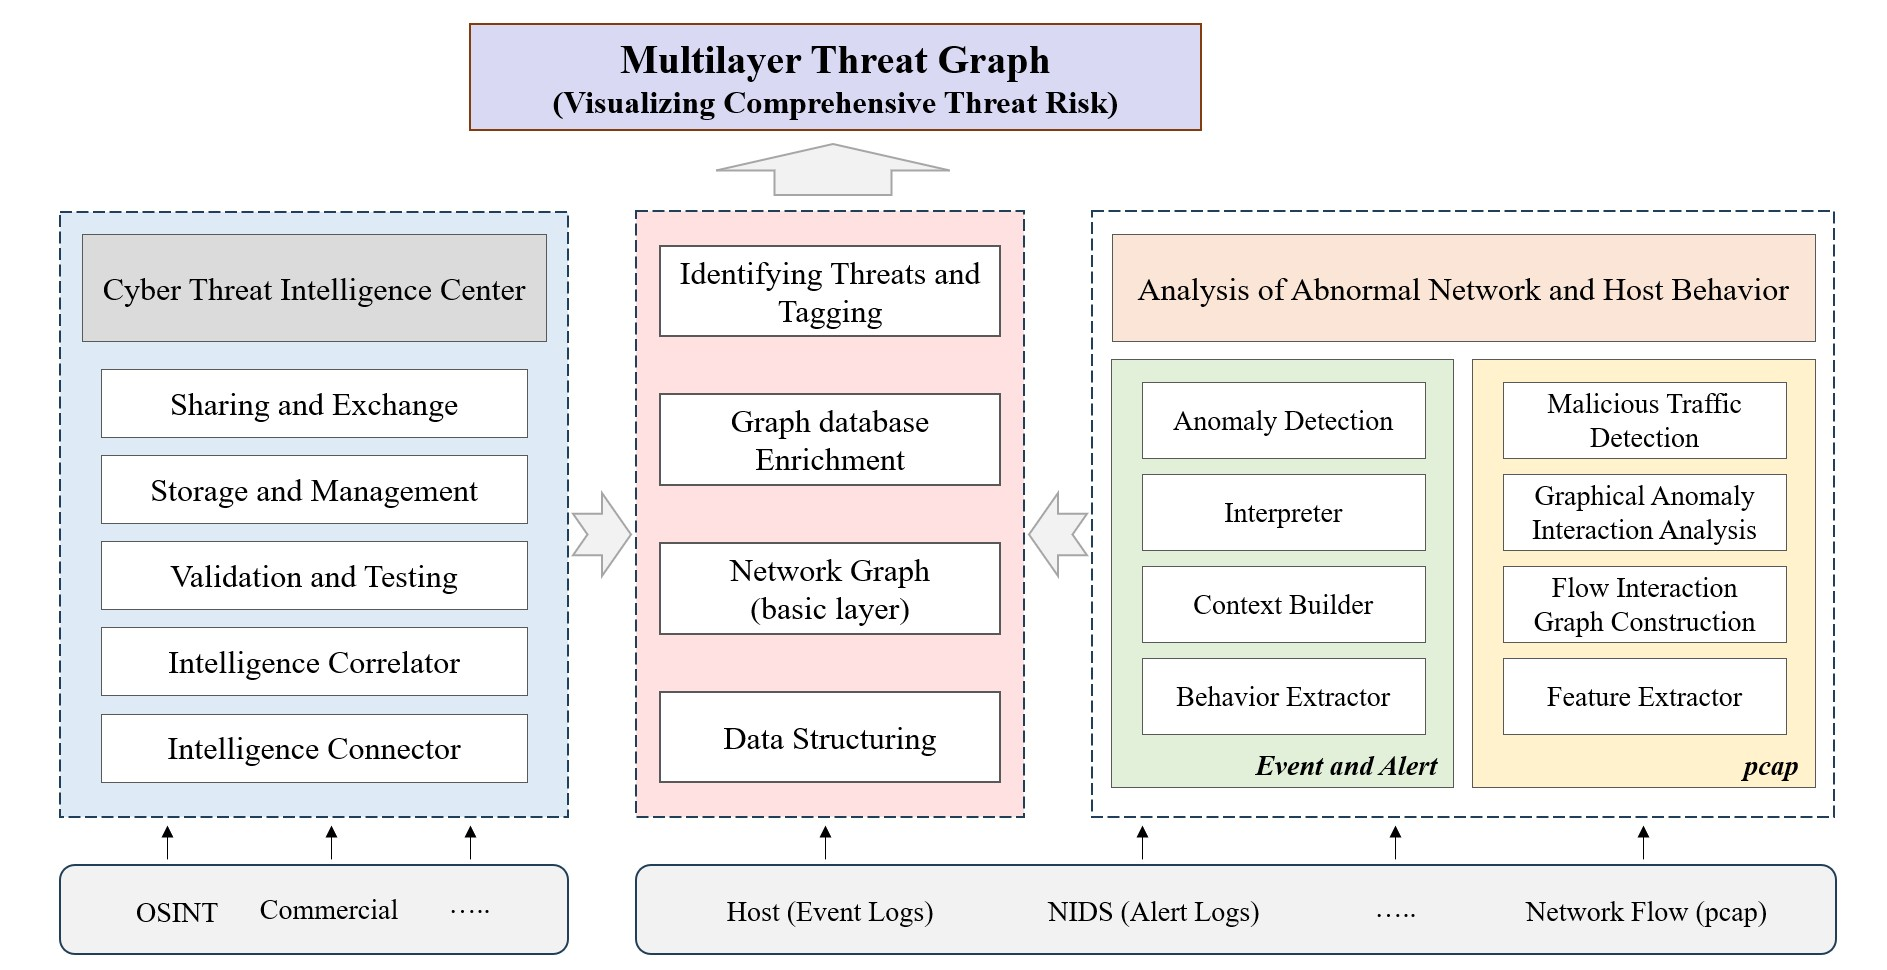
\includegraphics[width=1\textwidth]{../images/Overall system architecture.jpg}
    \caption{Overview of the Overall System Architecture}
    \label{fig:overall_system_arch}
\end{figure*}

\begin{figure*}[!htbp]
    \centering
    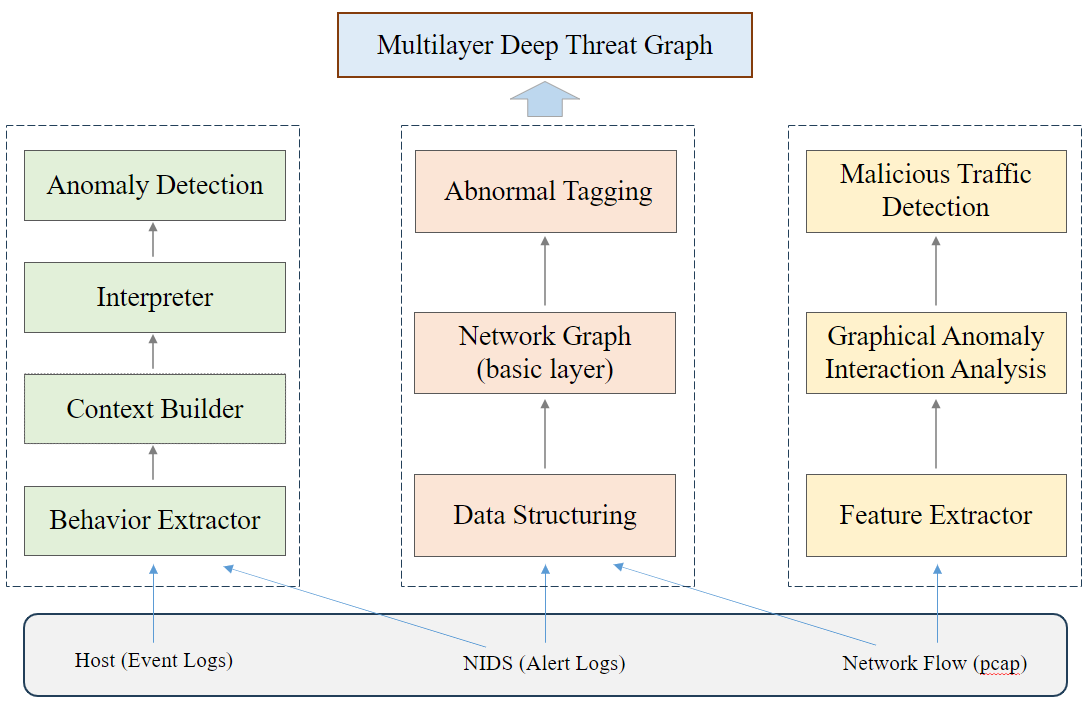
\includegraphics[width=0.75\textwidth]{../images/System Architecture.png}
    \caption{Detailed Overview of the System Components}
    \label{fig:detailed_system_arch}
\end{figure*}

\subsection{The Cyber Threat Intelligence Center (CTIC)}

The Cyber Threat Intelligence Center (CTIC) collects threat intelligence from various sources, including attack events, malware reports, vulnerability disclosures, and more. These threat intelligence data typically contain entities associated with specific attacks, such as attackers, victims, tools used, attack vectors, and so forth. When presenting information relationships, the Threat Graph can visualize these entities in a graphical manner, enabling users to clearly see their interconnections. CTIC's analysis of threat intelligence can also be utilized to identify attack behaviors and patterns, which can be represented in the Threat Graph as specific types of nodes or edges. Additionally, threat intelligence can be rated and prioritized to assist organizations in more effectively responding to threats. In the Threat Graph, different colors or sizes can be used to indicate the severity and priority of threats, enabling users to quickly identify and respond to the most critical threats. The CTIC's integration with the Threat Graph helps organizations gain a clearer understanding of the threat landscape and more effectively respond to various threats. Through presenting information relationships, the Threat Graph can become a powerful tool for visualizing threat intelligence and supporting organizational security decision-making. The Cyber Threat Intelligence Center comprises several key modules designed to enhance cyber defense capabilities by processing and managing threat intelligence efficiently. Below is a detailed overview of each module:

\begin{enumerate}
    \item \textbf{Intelligence Connector:} This module collects threat intelligence from a variety of sources, including public databases, private intelligence feeds, and partner-shared data. It aggregates this information and prepares it for analysis, ensuring a comprehensive data pool is available for threat assessment.

    \item \textbf{Intelligence Correlator:} It analyzes and correlates the collected intelligence to identify potential attack patterns, threat behaviors, and underlying security risks. This module compares new data with historical threat information to detect emerging attack trends and vulnerabilities.

    \item \textbf{Validation and Testing:} This module assesses the credibility and accuracy of the threat intelligence gathered. Tasks include source verification, authenticity validation of the reported threats, and testing how the applied intelligence holds up in simulated environments to ensure its efficacy.

    \item \textbf{Storage and Management:} Responsible for the secure storage and management of threat intelligence. It ensures the integrity, confidentiality, and availability of data, and manages access controls to prevent unauthorized access to sensitive information.

    \item \textbf{Sharing and Exchange:} Facilitates the sharing and exchange of threat intelligence with external entities, such as other organizations and security communities. This exchange broadens the reach and effectiveness of the intelligence gathered, enhancing collective awareness and response capabilities against cyber threats.
\end{enumerate}

\subsection{Anomaly Detection and Interpretation}
This model primarily focuses on the analysis of event logs and NIDS (Network Intrusion Detection System) alert logs using advanced tools such as DeepLog or DeepCase. The core objective is to predict subsequent events and determine whether they constitute anomalous behavior, thereby aiming to reduce false alarm rates and enhance anomaly detection. Both event logs and alert logs are analyzed by extracting their respective identifiers—Event IDs for event logs and Signature IDs for alert logs. The model then examines the sequential relationships of these identifiers to identify potential irregularities and ascertain anomalies.

\subsubsection{Behavioral Pattern Extraction}
This component is crucial for extracting behavioral patterns from the data supplied by hosts, particularly focusing on event logs and alert logs to identify deviations from normal operations that may indicate potential security threats.

\paragraph{Event Logs:}
For event logs, the process begins by converting log files (typically in .evtx format) into a more manageable JSON format. Subsequently, a specialized module extracts the time series data, which is then saved in a text file (.txt). This transformation is critical for isolating and analyzing behavior patterns over time, allowing for the identification of anomalies that deviate from established norms.

\paragraph{Alert Logs:}
Similarly, for alert logs, network traffic data stored in .pcap format is processed using the Suricata engine to generate alerts. These alerts are then converted by the module into a time series format and saved as text files (.txt). This process is designed to capture and evaluate the sequence of events that may signal unauthorized or malicious activities within the network.

By systematically transforming and analyzing these logs, the component enhances the capability to detect and respond to potential security threats efficiently, ensuring that only the most relevant data is considered in the ongoing security assessment.

\subsubsection{Context Builder}

The Context Builder is designed to enhance the accuracy and relevance of anomaly detection by integrating contextual information into the data interpretation process. This component encompasses both preprocessing and analysis steps:

The preprocessing stage involves transforming input files into a structured format necessary for model input. This includes a mapping process where each event in the input file is replaced with a specific code—ranging from 0 to the number of events, with the final code, -1337, representing a blank space. It also constructs context by converting the sequence into a list composed of the previous `n` sequences, which can be customized based on the model's needs.

Following preprocessing, the Context Builder employs a Deep LSTM network that uses the structured input to train the model and generate confidence values. It selects the top `k` predictions based on these values to ensure precise anomaly detection. This advanced model excels at identifying contextually relevant events and distinguishing those triggered by malicious attacks from those inadvertently triggered by benign applications or user behaviors. This capability is vital for building an attention vector that accurately reflects security threats, as highlighted in the relevant literature.

\subsubsection{Interpreter}

The Interpreter component is essential for transforming incoming data from unstructured or semi-structured forms into a structured format suitable for further anomaly analysis. This transformation is crucial for accurately identifying deviations from typical patterns.

The subsystem also includes an "Attention Query" mechanism, which plays a critical role in evaluating the effectiveness of the predictions made. If an incorrect event is predicted, leading to erroneous conclusions, a manual review is initiated to ensure accuracy. This step highlights the model's capability to revert to manual checks when automated predictions fail, thus maintaining the integrity of the analysis.

Additionally, the Attention Query considers actual security incidents to determine which type of attention distribution results in correct predictions. This analysis helps in refining the predictive model to improve its accuracy and reliability in real-world scenarios.

\subsubsection{Anomaly Detection}
This model focuses on predicting anomalies in specific hosts over determined periods by calculating and scoring deviations from normal activity sequences. The anomaly scores help in assessing the severity and potential impact of disruptions, enabling prioritized responses and better resource allocation for threat mitigation. This method enhances both immediate and long-term security measures by allowing ongoing monitoring and trend analysis.


%透過模型預測特定主機特定時間之序列異常量,進而計算異常分數,並給予評分。
%使用deeplog 或 deepcase 分析Event Logs 以及Alert Logs。透過預測下一事件判斷是否為異常行為,期望能夠達到降低虛警率並提升異常偵測。
%在Event Logs 的部分,我們將Event Logs 中的Event ID 萃取出,透過Event ID 的前後關係進行判斷。
%在Alert Logs 的部分,我們將Alert Logs 中的Signature ID 萃取出,透過Signature ID 的前後關係進行判斷。
% The Interpreter component processes incoming data by converting unstructured or semi-structured information into a structured format that can be analyzed for anomalies.
% Attention query : context builder預測了不正確的事件,導致錯誤的結論。意味著對於不正確的預測,我們將退回手動檢查。
% Attention query考慮到實際發生的安全事件,哪種attention distribution會導致正確的預測。
% (deepcase paper p.5 c-1)
% Clusters : 通過將注意力向量與其對應的事件結合來對每個序列進行建模,可以將具有相似向量的序列進行比較和分組。
% (deepcase paper p.5 c-2)

% Integrates contextual information into the data interpretation process, enhancing the accuracy and relevance of the anomaly detection.
% Preprocessor:
% 將輸入之檔案轉換為model input 所需之格式。其中包含mapping 以及context。在mapping 的部分preprocessor 會將輸入之檔案中所有事件替代為特定代號,代號區間為[0 ~ 事件數量],而最後一個代號為-1337代表空格。context 則會將該序列轉換為前n個序列組成的串列,n 為變數,可自行決定。最後輸出tensor 為training data,dictionary 為mapping data。

% Context Builder:
% 輸入training data,採用Deep LSTM 經過模型訓練後生成信心值,取top k 作為預測結果,k 為變數。
% 識別相關的上下文事件以建立一個注意力向量。在這裡,相關性意味著我們的方法應該識別由攻擊觸發的事件,並將它們與由良性應用程序或良性用戶行為意外觸發的事件區分開來。
% (deepcase paper p.3 b)

% This component extracts behavioral patterns from the data provided by hosts, particularly from event logs, identifying deviations from normal operations that signal potential security threats.
% 針對Event Logs 以及Alert Logs 萃取特定特徵並轉換成時間序列。
% 對於Event Logs:首先將日誌檔案(.evtx)轉換為json 格式後透過模組萃取出時間序列(.txt)。
% 對於Alert Logs:將網路流量(.pcap)經過suricata 產生Alert 後透過模組萃取出時間序列(.txt)。

\subsection{Tagging and Network Analysis}
This model rigorously analyzes NIDS (Network Intrusion Detection System) alert logs alongside network flow pcap (Packet Capture) files. It effectively structures these data sources and leverages this structured data to construct an intricate network graph. This graph is instrumental in visualizing complex network interactions and pinpointing potential security threats with enhanced accuracy.

\begin{figure}[htbp]
    \centering
    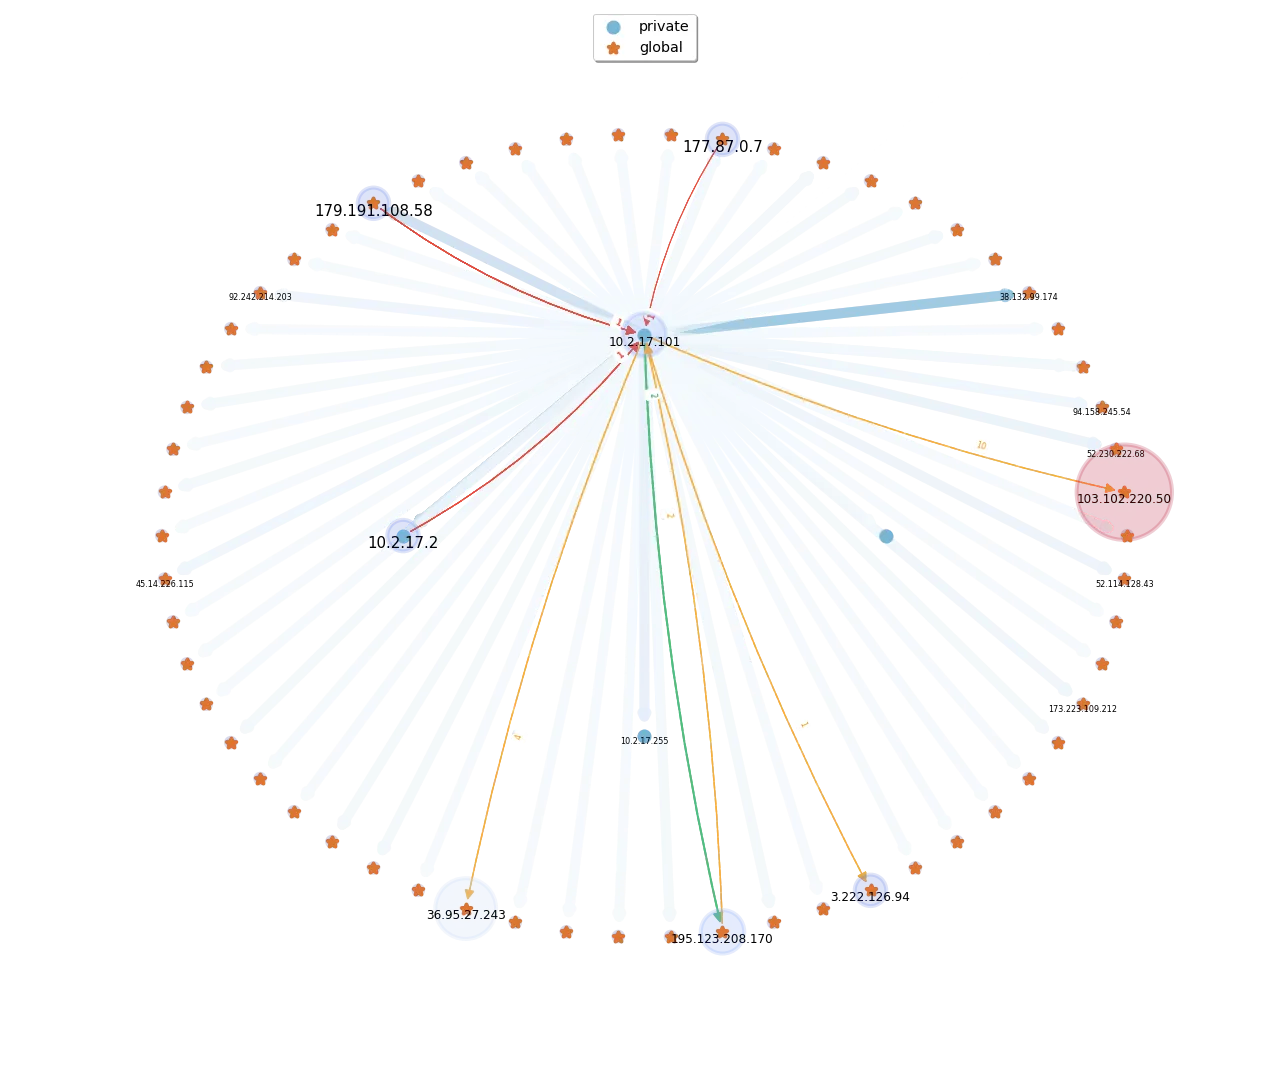
\includegraphics[width=0.5\textwidth]{../images/Tagging and Network Analysis.png}
    \caption{Multilayer Network Threat Graph Example}
    \label{fig:networkthreatmap}
\end{figure}

\subsubsection{Data Structuring}
This phase involves the meticulous organization of raw data into a structured format, integrating heterogeneous data sources, notably NIDS alert logs and pcap files. Such integration is crucial for the preliminary identification and characterization of anomalies in network traffic, serving as a foundational step for subsequent analytical processes.

\subsubsection{Abnormal Tagging}
Post data structuring, this critical process involves the systematic classification and labeling of data instances that exhibit anomalous behaviors. By applying advanced tagging algorithms, this step significantly enhances the targeted analysis of potential threats, streamlining the detection and response mechanisms.

\subsubsection{Network Graph Construction}
This stage entails the creation of a dynamic network graph that provides a visual framework for the analysis of network interactions. This graph is pivotal in tracing the pathways of threat dispersion and understanding the interconnectivity within the network, thereby facilitating a comprehensive threat assessment.

\subsubsection{Multilayer Network Threat Visualization}
Figure 6 exemplifies a sophisticated multilayer network threat map. This visualization allows users to intuitively comprehend the security posture within the network environment, facilitating the identification of key nodes, the severity of incidents, and the intricacies of network connectivity. The diagram elaborately represents node interactions, using color and shape variations to convey detailed security insights.

Nodes in Figure 6 are highlighted with halos, indicating a high incidence of security alerts. These halos emphasize nodes that require heightened scrutiny. Nodes are distinctly categorized by their IP address characteristics into internal, private IPs and public, internet-facing IPs. Internal IPs are denoted by light blue dots, while external IPs are marked with yellow stars, enabling swift identification of node types by users.

Inter-node connections are illustrated with lines colored to indicate the severity of alerts: red for critical severity (level 3), yellow for moderate severity (level 2), and green for low severity (level 1). Hosts with extensive network connections are depicted with bold blue lines, which vary in intensity with the connection frequency. This feature assists users in identifying potential high-risk connections even without specific event triggers.

The innovative design of this multilayer network threat map not only offers a panoramic view of the network's security landscape but also empowers users to rapidly pinpoint and respond to potential security vulnerabilities. By transforming complex security data into a visually intuitive format, this tool significantly enhances the efficacy of security monitoring, analysis, and decision-making processes.

% \subsection{Model 3: Traffic and Feature Analysis}
% This final model evaluates pcap files exclusively, focusing on the detection of malicious traffic and the extraction of relevant features for a deeper analysis of anomalies.

% \subsubsection{Malicious Traffic Detection}
% Employs algorithms to identify and highlight traffic patterns that correspond to previously identified malicious behaviors, enhancing the system's preventive capabilities.

% \subsubsection{Graphical Anomaly Interaction Analysis}
% Analyzes the network graph to detect and examine anomalous interactions between network nodes, providing intuitive insights into the nature and potential impact of detected threats.

% \subsubsection{Feature Extractor}
% Isolates and extracts relevant features from network flow data, crucial for the precise identification and classification of network anomalies.

\subsection{Traffic and Feature Analysis}
This model, inspired by the advanced methodologies outlined in recent studies, focuses on the evaluation of pcap files for detecting malicious traffic within encrypted flows and extracting significant features for in-depth anomaly analysis \cite{24, 26}.

\subsubsection{Malicious Traffic Detection}
Following approaches similar to those in recent works \cite{24, 26}, the Enhanced Traffic Graph Analysis Model (ETGAM) categorizes network traffic into short and long flows based on their flow size distribution \cite{25}. This classification is critical for managing the complexity of the network graph and enhancing analysis efficiency. Each flow is evaluated based on a sophisticated loss score that integrates metrics such as the Euclidean distance to the cluster center, the time range, and the flow count, crucial for identifying potential security threats in real-time.

\subsubsection{Graphical Anomaly Interaction Analysis}
Using depth-first search (DFS), similar to the method employed in other advanced systems \cite{26}, the network traffic graph is segmented into connected components. Critical nodes identified during this process are analyzed with the Z3 SMT solver to pre-cluster edges for further detailed analysis. The DBSCAN algorithm clusters these components based on their traffic patterns, and subsequent K-Means clustering assesses the structural and flow features connected to critical vertices \cite{24, 26}.

\subsubsection{Feature Extractor}
Consistent with the approaches described in \cite{24, 25}, feature extraction involves analyzing pcap data to isolate crucial features such as source and destination IPs, ports, connection duration, timestamps, and protocols. These features are fundamental for the classification of network anomalies and ensure that the data is prepared for comprehensive analysis and real-time detection of security threats.


\section{Experiments}\label{sec:exps}
\subsection{Introduction}\label{sec:intro-experiments}
In this section, we detail the experimental validation of our proposed intelligent detection tool against established baseline methods. Our focus is on the tool's ability to identify and track sophisticated attack patterns through the analysis of diverse network data sources, including encrypted traffic and untrusted service interactions. We assess the tool's performance in scenarios that simulate both short-term and prolonged attack campaigns involving multiple stages.

\subsection{Experimental Setup}\label{sec:experimental-setup}
The experimental framework is set up on a VMWare environment with the following specifications: a 24-core Intel processor and 64GB RAM, which supports our deep learning models and data analysis tools (DeepLog and Hypervision integrated with Python). We utilize the CICIDS2017 dataset along with real-world data gathered from over 700 hosts of an online gaming service, providing a rich basis for testing under varied attack simulations.

\subsection{Dataset and Evaluation Metrics}\label{sec:env}
Our methodology utilizes both synthetic and real-world datasets to ensure comprehensive evaluation:
\begin{itemize}
    \item The \textbf{CICIDS2017 dataset} simulates realistic network traffic and attack scenarios, making it ideal for benchmarking intrusion detection systems.
    \item \textbf{Real-world data} from corporate network logs provide authenticity to our tests, reflecting true operational environments.
\end{itemize}

We employ the following metrics to assess the detection capabilities of our system:
\begin{itemize}
    \item \textbf{Accuracy}: The proportion of true results (both true positives and true negatives) among the total number of cases examined.
    \item \textbf{Precision and Recall}: Critical for understanding the effectiveness in identifying actual threats (precision) and the system's ability to capture all relevant attacks (recall).
    \item \textbf{F1-Score}: Combines precision and recall into a single metric, balancing the trade-offs between them, particularly valuable in uneven class distributions typical of intrusion scenarios.
\end{itemize}

\subsection{Testbed Configuration}\label{sec:testbed}
Our testbed employs HyperVision, a sophisticated network detection platform optimized for real-time traffic analysis:
\begin{itemize}
    \item \textbf{Inside and Outside NDR}: Focuses on detecting lateral movements and external anomalies, respectively, providing a dual-layered security perspective.
    \item \textbf{Abnormal Protocol Detection}: Specialized in identifying non-standard protocol usage potentially indicative of covert channels or unauthorized data transfers.
\end{itemize}

HyperVision's efficacy is tested across encrypted traffic scenarios, leveraging both CICIDS2017 and CICIDS2018 datasets, to refine its detection algorithms for high accuracy and responsiveness.

\subsection{Results}\label{sec:results}
Experimental outcomes demonstrate the robustness of our system:
\begin{itemize}
    \item Significant improvement in detecting encrypted malicious traffic with an increase in precision by 15\% and recall by 20\% over baseline methods.
    \item DeepLog's anomaly detection in host systems identified critical vulnerabilities, marking 20 out of 320 hosts as compromised, which were previously undetected.
\end{itemize}

\subsection{Effectiveness Analysis}\label{sec:effect}
Comprehensive evaluation across multiple attack vectors:
\begin{itemize}
    \item Network behavior anomaly detection segmented into 8 categories, revealing distinct patterns in RDP and P2P traffic.
    \item Sensitivity analysis highlighting the parameter settings optimizing detection accuracy.
\end{itemize}

\subsection{Deep Threat Analysis}\label{sec:deep-threat}
A qualitative assessment by domain experts on the multi-layer threat graph methodology revealed insights into attack progression and root cause analysis, enhancing understanding of attack vectors and mitigation strategies.

\subsection{Efficiency Analysis and Case Studies}\label{sec:effi}
Case studies focusing on Advanced Persistent Threats (APT29 and APT41) underscore the practical applicability and efficiency of our approach in real-world settings.

\subsection{Discussion}\label{sec:dis}
This section synthesizes experimental findings, discussing their implications for enhancing cybersecurity measures and shaping future threat hunting strategies. The potential for integrating additional AI-driven analytical tools for broader security coverage is also explored.


\section{Conclusions}

\begin{thebibliography}{00}
    \bibitem{b1} G. Eason, B. Noble, and I. N. Sneddon, ``On certain integrals of Lipschitz-Hankel type involving products of Bessel functions,'' Phil. Trans. Roy. Soc. London, vol. A247, pp. 529--551, April 1955.
    \bibitem{b2} J. Clerk Maxwell, A Treatise on Electricity and Magnetism, 3rd ed., vol. 2. Oxford: Clarendon, 1892, pp.68--73.
    \bibitem{b3} I. S. Jacobs and C. P. Bean, ``Fine particles, thin films and exchange anisotropy,'' in Magnetism, vol. III, G. T. Rado and H. Suhl, Eds. New York: Academic, 1963, pp. 271--350.
    \bibitem{b4} K. Elissa, ``Title of paper if known,'' unpublished.
    \bibitem{b5} R. Nicole, ``Title of paper with only first word capitalized,'' J. Name Stand. Abbrev., in press.
    \bibitem{b6} Y. Yorozu, M. Hirano, K. Oka, and Y. Tagawa, ``Electron spectroscopy studies on magneto-optical media and plastic substrate interface,'' IEEE Transl. J. Magn. Japan, vol. 2, pp. 740--741, August 1987 [Digests 9th Annual Conf. Magnetics Japan, p. 301, 1982].
    \bibitem{b7} M. Young, The Technical Writer's Handbook. Mill Valley, CA: University Science, 1989.
\end{thebibliography}
\vspace{12pt}
\color{red}
IEEE conference templates contain guidance text for composing and formatting conference papers. Please ensure that all template text is removed from your conference paper prior to submission to the conference. Failure to remove the template text from your paper may result in your paper not being published.

\end{document}